\documentclass[letterpaper, conference]{IEEEtran}
\IEEEoverridecommandlockouts

% Strict margin enforcement and text wrapping
\usepackage[letterpaper, top=0.75in, bottom=1in, left=0.625in, right=0.625in]{geometry}
\usepackage{microtype}

\usepackage{cite}
\usepackage{amsmath,amssymb,amsfonts}
\usepackage{algorithm}
\usepackage{algorithmic}
\usepackage{graphicx}
\usepackage{textcomp}
\usepackage{xcolor}
\usepackage{booktabs}
\usepackage{multirow}
\usepackage{array}
\usepackage{url}
\usepackage{subcaption}
\usepackage{caption}
\usepackage{placeins}
\usepackage{colortbl}
% \usepackage{stfloats}  % not installed in all TeX distributions; no [b] figure* is used
\usepackage{tikz}
\usetikzlibrary{arrows.meta,shapes.geometric,positioning,fit,backgrounds,calc}

\definecolor{llmblue}   {RGB}{76,114,176}
\definecolor{vitgreen}  {RGB}{85,168,104}
\definecolor{vlmred}    {RGB}{196,78,82}
\definecolor{fedorange} {RGB}{204,185,116}
\definecolor{fedpurple} {RGB}{129,114,178}
\definecolor{outyyellow}{RGB}{255,242,204}
\definecolor{smallgray} {RGB}{220,220,220}

\graphicspath{{omnimed_plots/}}

\tikzset{
  mainbox/.style={draw, rounded corners=4pt, align=center,
                  minimum height=0.75cm, text width=#1,
                  font=\footnotesize, inner sep=4pt},
  mainbox/.default=2.4cm,
  llmbox/.style ={mainbox, fill=llmblue!30,  draw=llmblue!80!black},
  vitbox/.style ={mainbox, fill=vitgreen!30, draw=vitgreen!80!black},
  vlmbox/.style ={mainbox=5.2cm, fill=vlmred!25, draw=vlmred!80!black,
                  minimum height=1.0cm},
  fedbox/.style ={mainbox=1.9cm, fill=fedpurple!40, draw=fedpurple!80!black},
  outbox/.style ={mainbox=4.5cm, fill=outyyellow, draw=yellow!70!black},
  sbox/.style   ={draw, rounded corners=2pt, fill=smallgray,
                  minimum height=0.5cm, align=center,
                  font=\scriptsize, inner sep=3pt, text width=1.8cm},
  arr/.style    ={-{Stealth[length=5pt]}, thick},
  darr/.style   ={-{Stealth[length=5pt]}, thick, dashed},
}

\begin{document}
\renewcommand{\arraystretch}{0.85}
\setlength{\abovecaptionskip}{0pt}
\setlength{\belowcaptionskip}{0pt}

\setlength{\columnsep}{0.25in}

\renewcommand{\dbltopfraction}{0.9}
\renewcommand{\topfraction}{0.9}

\title{OmniMed-FL: A Robust Multimodal Federated Learning Framework for Clinical Diagnosis}

\author{
\IEEEauthorblockN{$^1$Ayush Debnath, $^{2,3,4}$Ruelia Saha, $^{2}$Sudip Misra}

\IEEEauthorblockA{$^1$Department of Mechanical Engineering\\
Indian Institute of Technology Kharagpur, India-721302}

\IEEEauthorblockA{$^2$Computer Science \& Engineering Department\\
IIT (Indian Institute of Technology) Kharagpur, India-721302}

\IEEEauthorblockA{$^3$KTH Royal Institute of Technology, Stockholm, Sweden}

\IEEEauthorblockA{$^4$SRM University- AP, India}

Email: \{ayush.d@kgpian.iitkgp.ac.in, ruelia.saha.rs@gmail.com, sudipm@iitkgp.ac.in\}
}

\maketitle

\begin{abstract}
Clinical diagnosis requires medical images and patient records together, yet most machine learning systems model one modality, and privacy rules such as HIPAA and GDPR block hospitals from pooling records centrally---leaving secure cross-institutional fusion an open problem. We propose OmniMed-FL, a multi-modal federated learning framework for multi-class clinical condition classification (Normal, Pneumonia, COVID-19, Pleural Effusion, Cardiomegaly). The framework benchmarks five LLM text encoders, five Vision Transformer (ViT) image encoders, and eight VLM fusion strategies under FedAvg with non-IID Dirichlet(alpha=1.0) partitioning across 5 hospital clients. An anti-collapse stack of balanced batch sampling, entropy diversity regularization and adaptive early abort prevents majority-class collapse: diversity dips are transient and all 18 variants recover full five-class diversity by epoch~5. DistilBERT achieves an F1 score of 0.934 on text; ViT-Base achieves an F1 score of 0.664 on images; Concat VLM fusion achieves an F1 score of 0.956, a gain of $+$2.2 F1 points over the best unimodal baseline. Under non-IID conditions, federated training retains 99.1\% of centralized Macro F1 averaged over the three branches: Fed-VLM (0.956) matches its centralized counterpart and Fed-LLM (0.953) exceeds its own (0.934), while the image-only branch loses 4.8\%. Against the 31 published systems compiled in Table~IV, Fed-VLM is the strongest federated entry and second overall behind a centralized EfficientNet-B7 (0.980), though those systems use different corpora so the positioning is indicative only. A FAISS-indexed retrieval layer returns the correct condition as its top-1 match for all five probe queries, at cosine similarities of 0.66--0.85.
\end{abstract}

\begin{IEEEkeywords}
Multimodal Federated Learning, Vision-Language Models, Clinical Condition Classification, E-Health, Privacy-Preserving AI, Multimodal Learning, RAG, Vision Transformer, Large Language Model
\end{IEEEkeywords}

% ─────────────────────────────────────────────────────────────────────────────
\section{Introduction}
% ─────────────────────────────────────────────────────────────────────────────

\IEEEPARstart{C}{linical} condition classification, which covers
distinguishing normal presentations from acute infections, fluid
accumulation, and structural cardiac pathology, is central to timely patient intervention. Most existing automated diagnostic systems rely on a single type of data. They use either CNNs or vision transformers to analyze chest radiographs~\cite{Rajpurkar2017,Irvin2019}, or language models to process information from electronic health records.
Neither source of information is sufficient on its own. Image-based models can overlook important clinical context, such as elevated BNP levels or a history of viral exposure. Text-based models cannot directly capture radiological findings such as bilateral ground-glass opacities or a pleural fluid meniscus.

Deploying such systems in healthcare is also challenging because patient data is spread across hospitals, clinics, and diagnostic centres, while privacy regulations such as HIPAA and GDPR restrict the centralised collection of sensitive medical records. Federated Learning (FL) provides a practical alternative by allowing institutions to train a shared model through locally computed parameter updates without exchanging raw patient data. However, most existing FL methods for clinical applications still focus on a single modality and do not make use of the textual notes that clinicians routinely record alongside medical images~\cite{Sheller2020,Dou2021,Kaissis2021}.

%This leaves the field at an impasse. 
This highlights an important gap in current clinical AI systems. Physicians often rely on multiple sources of information when making a diagnosis, yet existing frameworks either sacrifice patient privacy or fail to combine these modalities effectively. Centralised vision-language models require sensitive patient data to be pooled at a common location, creating privacy and regulatory concerns, while existing federated approaches~\cite{Sheller2020,Kaissis2021} largely focus on medical images alone. To address this limitation, we developed OmniMed-FL, a federated multimodal framework that allows hospitals to collaboratively train accurate clinical models using both imaging and textual information without exposing raw patient data.


\subsection{Contribution}
The main \textit{contributions} of this paper are as follows:
\begin{itemize}
\item We study how combining medical images with electronic health records can improve diagnosis in a federated setting. The results show that using both modalities gives better performance than relying on images or text alone.

\item We prepare a controlled clinical dataset in which similar information appears across different disease classes. This reduces the chance of the model making predictions from a few obvious keywords and requires it to use information from both the image and the clinical record.

\item We evaluate OmniMed-FL under non-IID data distributions that reflect differences between participating hospitals. The federated model achieves performance close to centralized training while keeping the original patient data within each institution.
\end{itemize}


% ─────────────────────────────────────────────────────────────────────────────
\section{Related Work}

\subsection{Medical Image Classification}
Early work on automated diagnosis mainly treated radiology as an image classification problem. Rajpurkar \textit{et al.}~\cite{Rajpurkar2017} and Irvin \textit{et al.}~\cite{Irvin2019} showed the effectiveness of CNN-based models for chest X-ray classification in centralized settings. Later work explored Vision Transformers~\cite{Dosovitskiy2021,Liu2021swin}, which capture broader spatial relationships within an image. Although these approaches achieve strong classification performance, they generally rely on centrally collected datasets and do not make use of the clinical notes that often accompany medical images.

\subsection{Federated Clinical Learning}
Federated Learning (FL) has been studied as a way to train clinical models without moving patient data outside individual institutions. Sheller \textit{et al.}~\cite{Sheller2020} applied FedAvg in a decentralized medical imaging setting and Dou \textit{et al.}~\cite{Dou2021} validated a federated model across national sites, while Kaissis \textit{et al.}~\cite{Kaissis2021} considered additional privacy protection through differential privacy. Such methods allow hospitals to participate in joint model training while keeping raw data locally. However, most of these approaches are designed around a single modality and mainly consider medical images.

\subsection{Vision-Language Models in Healthcare}
Another line of work has focused on combining medical images with textual information. Models such as BiomedCLIP~\cite{Zhang2023biomedclip}, LLaVA-Med~\cite{Li2023llavamed}, and MedCLIP~\cite{Wang2022medclip} learn relationships between medical images and associated reports or clinical text. This allows the model to use information from both modalities rather than treating the image independently. However, these models are generally developed and trained in centralized settings, which makes their direct use across hospitals with isolated patient data difficult.

\textbf{Synthesis:}
As summarized in Table~\ref{tab:relwork}, existing work generally addresses either multimodal learning or decentralized training. Vision-language models make use of both image and text information, whereas federated clinical models allow training across institutions without sharing raw data. There is comparatively limited work combining both aspects within the same framework. OmniMed-FL is designed to address this gap by incorporating image-text fusion into a federated learning setup for clinical diagnosis.


\begin{table}[t]
\caption{Positioning vs.\ Related Work.}
\label{tab:relwork}
\centering\footnotesize
\setlength\tabcolsep{6pt}
\begin{tabular}{lcccc}
\toprule
 & \multicolumn{2}{c}{\textbf{Modality}} & \multicolumn{2}{c}{\textbf{Framework}}\\
\cmidrule(lr){2-3}\cmidrule(lr){4-5}
\textbf{Work} & \textbf{Img} & \textbf{Text} & \textbf{FL} & \textbf{VLM}\\
\midrule
CheXNet~\cite{Rajpurkar2017}       & \checkmark & $\times$ & $\times$ & $\times$ \\
Sheller 2020~\cite{Sheller2020}    & \checkmark & $\times$ & \checkmark & $\times$ \\
Kaissis 2021~\cite{Kaissis2021}    & \checkmark & $\times$ & \checkmark & $\times$ \\
BiomedCLIP~\cite{Zhang2023biomedclip} & \checkmark & \checkmark & $\times$ & \checkmark \\
MedCLIP~\cite{Wang2022medclip}     & \checkmark & \checkmark & $\times$ & \checkmark \\
\midrule
\rowcolor{vlmred!20}
\textbf{OmniMed-FL (ours)}         & \checkmark & \checkmark & \checkmark & \checkmark \\
\bottomrule
\end{tabular}
\end{table}

% ─────────────────────────────────────────────────────────────────────────────
\section{System Design}
% ─────────────────────────────────────────────────────────────────────────────

\subsection{Architecture}

Figure~\ref{fig:arch} shows the overall OmniMed-FL pipeline. Clinical notes are first tokenized using WordPiece with a maximum sequence length of 128 tokens, while chest radiographs are resized to $224{\times}224$ and normalized using ImageNet statistics. The text encoder produces a feature vector $\mathbf{h}_t\!\in\!\mathbb{R}^{256}$ using the \texttt{[CLS]} representation, whereas the image encoder generates $\mathbf{h}_v\!\in\!\mathbb{R}^{512}$ using adaptive average pooling.

The two feature representations are then combined in the VLM module. We evaluate eight fusion methods: Concatenation, Cross-Attention, Gated Fusion, CLIP, Flamingo, BLIP-2, CoCa, and Unified-IO. Each method produces a joint representation $\mathbf{h}_f$, which is passed to a linear classifier for five-class prediction.

We included both simple and more complex fusion methods to study whether additional attention mechanisms provide enough benefit to justify their computational cost in a federated hospital setting. As shown in Figure~\ref{fig:fusion_comp}, seven of the eight fall within a 1.0-point band (0.946--0.956) and all seven exceed the best unimodal encoder, with plain concatenation highest. Since each variant was run once, that spread is not a defensible ordering: the benefit comes from having both modalities rather than from the fusion operator, which favours the cheapest option. CoCa (0.662) does not converge within this budget.


% \begin{figure}[t]
% \centering
% 
\includegraphics[width=0.98\columnwidth]{plot03_vlm_fusion_comparison}
% \caption{Benchmark of 8 VLM fusion strategies. Seven of the eight lie within 1.0 point of each other (0.946--0.956) and all seven exceed the best unimodal encoder (dashed lines); Concat is highest and Gated lowest of the seven. CoCa (orange) does not converge under the same budget.}
% \label{fig:fusion_comp}
% \end{figure}

\begin{figure}[t]
\centering
\resizebox{0.98\columnwidth}{!}{%
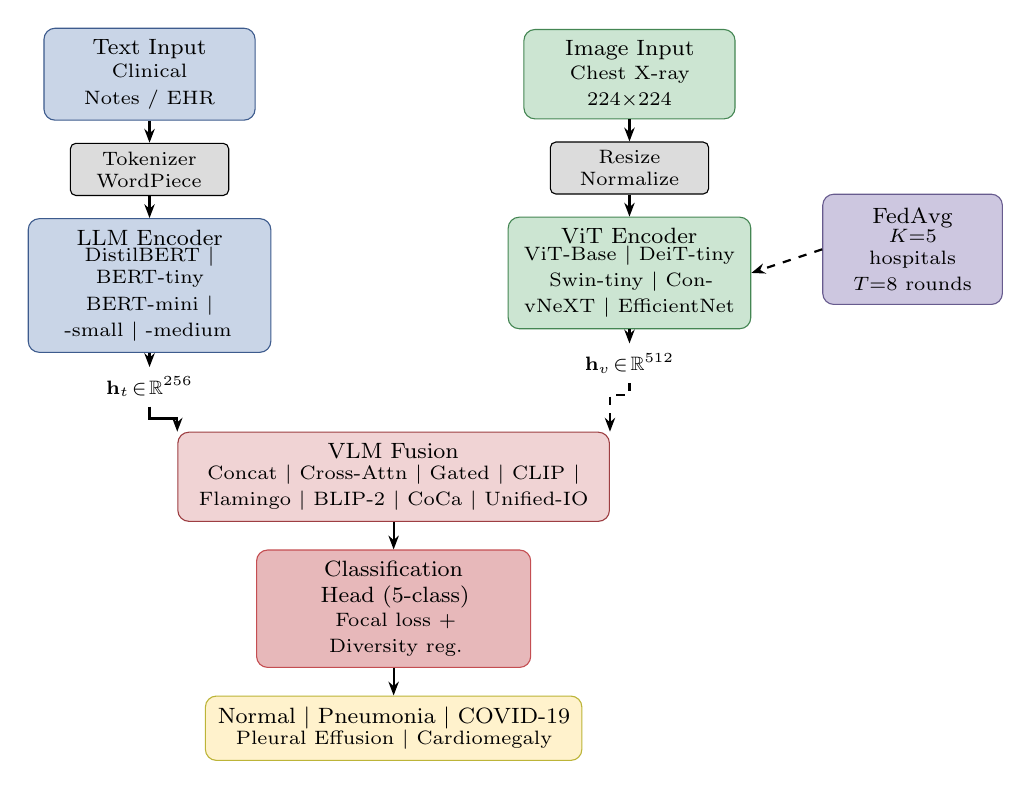
\begin{tikzpicture}[node distance=0.45cm]
  \node[llmbox] (ti)  {Text Input\\[-1pt]{\scriptsize Clinical Notes / EHR}};
  \node[sbox, below=0.28cm of ti] (tok) {Tokenizer\\WordPiece};
  \node[llmbox, below=0.28cm of tok, text width=2.8cm, minimum height=1.0cm]
        (llm) {LLM Encoder\\[-2pt]
               {\scriptsize DistilBERT $|$ BERT-tiny\\
               BERT-mini $|$ -small $|$ -medium}};
  \node[font=\scriptsize, below=0.18cm of llm] (ht)
        {$\mathbf{h}_t\!\in\!\mathbb{R}^{256}$};

  \node[vitbox, right=3.4cm of ti] (ii) {Image Input\\[-1pt]
                                         {\scriptsize Chest X-ray $224{\times}224$}};
  \node[sbox, below=0.28cm of ii] (aug) {Resize\\Normalize};
  \node[vitbox, below=0.28cm of aug, text width=2.8cm, minimum height=1.0cm]
        (vit) {ViT Encoder\\[-2pt]
               {\scriptsize ViT-Base $|$ DeiT-tiny\\
               Swin-tiny $|$ ConvNeXT $|$ EfficientNet}};
  \node[font=\scriptsize, below=0.18cm of vit] (hv)
        {$\mathbf{h}_v\!\in\!\mathbb{R}^{512}$};

  \node[fedbox, right=0.9cm of vit, yshift=0.3cm, minimum height=1.4cm,
        text width=2.0cm] (fed)
        {FedAvg\\[-1pt]{\scriptsize $K{=}5$\\hospitals\\$T{=}8$ rounds}};

  \node[vlmbox, below=1.0cm of llm, xshift=3.1cm, minimum height=0.95cm]
        (vlm) {VLM Fusion\\[-2pt]
               {\scriptsize Concat $|$ Cross-Attn $|$ Gated $|$ CLIP $|$
               Flamingo $|$ BLIP-2 $|$ CoCa $|$ Unified-IO}};

  \node[mainbox=3.2cm, fill=vlmred!40, draw=vlmred,
        below=0.35cm of vlm] (cls)
        {Classification Head (5-class)\\[-1pt]
         {\scriptsize Focal loss + Diversity reg.}};

  \node[outbox, below=0.35cm of cls] (out)
        {Normal $|$ Pneumonia $|$ COVID-19\\[-2pt]
         {\scriptsize Pleural Effusion $|$ Cardiomegaly}};

  \draw[arr](ti)--(tok);\draw[arr](tok)--(llm);\draw[arr](ii)--(aug);
  \draw[arr](aug)--(vit);\draw[arr](llm)--(ht);\draw[arr](vit)--(hv);
  \draw[arr](ht.south)--++(0,-0.15)-|(vlm.north west);
  \draw[darr](hv.south)--++(0,-0.15)-|(vlm.north east);
  \draw[arr](vlm)--(cls);\draw[arr](cls)--(out);
  \draw[darr](fed.west)--(vit.east);
\end{tikzpicture}%
}
\caption{OmniMed-FL architecture. LLM and ViT encoders process clinical
notes and chest X-rays; VLM fusion combines both modalities; FedAvg
coordinates $K{=}5$ hospital clients without transmitting raw patient data.}
\label{fig:arch}
\end{figure}

\begin{figure}[t]
\centering

\includegraphics[width=0.98\columnwidth]{plot03_vlm_fusion_comparison}
\caption{Benchmark of 8 VLM fusion strategies. Simple Concatenation (Concat) and Gated Fusion provide the best balance of Accuracy and Macro F1.}
\label{fig:fusion_comp}
\end{figure}

\begin{figure}[t]
\centering

\includegraphics[width=0.98\columnwidth]{plot02_vit_comparison}
\caption{Comparison of image backbones. The three attention-based backbones cluster at Macro F1 0.647--0.664; the two convolutional baselines fall to 0.32--0.34.}
\label{fig:vit_comp}
\end{figure}

\subsection{Encoding Specifications}
For the text branch, we use DistilBERT, which consists of 6 transformer layers with a hidden size of 768, 12 attention heads, and approximately 66 million parameters. The first four layers are kept frozen during training, while the remaining layers are fine-tuned on the clinical data. This reduces the number of trainable parameters while still allowing the model to adapt to medical terminology and task-specific patterns. For the image branch, we use ViT-Base/16 with 12 transformer layers, a hidden size of 768, 12 attention heads, and approximately 86 million parameters.
We selected ViT-Base/16 because it is the highest-scoring backbone in Figure~\ref{fig:vit_comp}, though its margin over Swin-tiny (0.664 vs.\ 0.661) is small enough that the two should be treated as equivalent here; the clear separation is between the attention-based backbones and the convolutional ones. The network splits incoming images into $16{\times}16$ token patches and prepends a learnable \texttt{[CLS]} token. For both modalities, a projection head maps the native hidden states to a shared latent space ($d=256$ or $512$) prior to concatenation or cross-attention fusion.

\subsection{Dataset and Clinical Corpus}

\textbf{Image data.}
We built the visual dataset by aggregating public chest X-ray collections and mapping them to our five target conditions. Our sources include the keremberke pneumonia dataset, Tawsifur's COVID-19 image set, and the NIH Chest X-ray dataset (which we filtered down from 14 labels to our specific 5). Whenever a class lacked enough real samples, we supplemented the training set with synthetic, X-ray-style images designed with specific pixel signatures---such as a bright lower-lobe patch for Pneumonia or a basal opacity gradient for Pleural Effusion. We normalized all images using ImageNet statistics and saved them as float16 tensors to cut memory usage in half. We balanced the corpus at 600 samples per class, yielding 3,000 images total, split 80/20 for training and validation.

\textbf{Clinical text data.}
Because real EHR data is difficult to source publicly, we built a template engine to generate 3,000 synthetic medical reports. We populated these reports using vocabulary pools mapped to specific observations, symptoms, and conditions. To reduce the chance of the model relying on obvious keywords, we use a 75\%/25\% mixed-to-clear slot ratio. The mixed samples contain overlapping or cross-class phrasing, which makes the text less directly indicative of the target class and encourages the model to use the full clinical context. All generated text is normalized, and any simulated patient identifiers are removed. The templates are also constructed so that the pathological descriptions in the text remain consistent with the corresponding findings in the paired X-ray. This provides a controlled setting for evaluating how effectively the fusion module combines information from the two modalities.

\label{sec:corpus}
\textbf{What this corpus does and does not support.}
Because the cross-modal alignment is known by construction, every variant sees identical data and differences between variants are attributable to the variant. The corpus is not a substitute for clinical data, and it bounds what the numbers mean. Template notes draw on a smaller, more regular vocabulary than dictated reports and reproduce none of their negation-scope errors, hedging, abbreviation drift or comorbidity structure; the images used to top up under-represented classes are pixel-pattern surrogates, not radiographs. Both make the modalities more separable than they would be in practice, and asymmetrically so---the text branch benefits more---so the modality gap we report is very likely an upper bound on the real one, and the absolute Macro F1 values are ceilings obtained under favourable conditions. What the corpus does support are the \emph{relative} comparisons: across modalities, across fusion strategies, and between federated and centralized training. Those are what we draw conclusions from.

\subsection{Experimental Setup}

\textbf{Hyperparameters.}
Each client model is trained locally using the AdamW optimizer. We use a learning rate of $2{\times}10^{-5}$ for the language encoder and $1{\times}10^{-4}$ for both the ViT and the fusion head. A linear warmup is applied during the first 10\% of the training iterations. Each client performs five local epochs ($E=5$) before sending its updated model parameters to the central server for aggregation. The coefficient of the diversity regularizer is set to $\lambda=0.1$ based on a grid search over values ranging from 0.01 to 0.5. All experiments are implemented in PyTorch 2.4 and run on NVIDIA A100 GPUs. Automatic Mixed Precision (AMP) is used to reduce training time and memory usage. The complete set of hyperparameters used across all clients is given in Table~\ref{tab:hyper}.

\textbf{Partitioning.}
To represent differences in data distributions across hospitals, we divide the dataset among clients using a Dirichlet non-IID partition. We set the concentration parameter to $\alpha=1.0$, which produces heterogeneous class distributions across clients. As a result, some clients may contain a larger proportion of Pneumonia cases, while others may contain more Normal or other diagnostic classes. This setting allows us to evaluate how well federated averaging performs when the local training distributions differ across participating hospitals. We note that $\alpha=1.0$ draws each client's class proportions uniformly from the probability simplex, which is a \emph{moderate} rather than an extreme heterogeneity setting: $\alpha\!\to\!\infty$ recovers the IID case and $\alpha\!\ll\!1$ produces the regime in which most clients see only one or two classes. It is the reference value used in the federated visual classification literature~\cite{Hsu2019}; results under smaller $\alpha$ are not reported here and are discussed in Section~\ref{sec:limits}.

\textbf{Rationale for Table~\ref{tab:hyper}.}
These values were fixed once and reused for all 18 variants, so no comparison is confounded by per-model tuning. $E{=}5$, $T{=}8$ follows from Figure~\ref{fig:conv}: the model is within one point of its final Macro F1 by round~3, so $T{=}8$ leaves margin past convergence while keeping synchronizations---and the cost in Section~\ref{sec:cost}---small. The rates differ by branch because $2{\times}10^{-5}$ is the standard range for a pretrained BERT-family encoder while the ViT projection and fusion head start from a task-agnostic or random init and need $1{\times}10^{-4}$; one rate for both under-trains the head. A batch of 32 is the largest holding both encoders at $224{\times}224$ in FP16 on one device and the smallest for which the balanced sampler can place several examples of each class per batch, a precondition for the diversity term to get a usable gradient. The $\lambda$ range $[0.01,\,0.5]$ brackets the regimes where the entropy term is negligible against the focal loss and where it dominates.

\begin{table}[t]
\caption{Global Hyperparameter Configuration.}
\label{tab:hyper}
\centering\footnotesize
\begin{tabular}{ll}
\toprule
\textbf{Parameter} & \textbf{Value} \\
\midrule
Local Epochs ($E$) & 5 \\
Federated Rounds ($T$) & 8 \\
Batch Size & 32 \\
LLM Learning Rate & $2 \times 10^{-5}$ \\
ViT Learning Rate & $1 \times 10^{-4}$ \\
Fusion Learning Rate & $1 \times 10^{-4}$ \\
Weight Decay & $0.01$ \\
Warmup Steps & 100 \\
Diversity Reg. ($\lambda$) & 0.1 \\
Dirichlet Alpha ($\alpha$) & 1.0 \\
Precision & FP16 (AMP) \\
\bottomrule
\end{tabular}
\end{table}

\begin{table}[t]
\caption{Macro F1 Scores Across All 18 Evaluated Variants}
\label{tab:performance_variants}
\centering
\footnotesize
\renewcommand{\arraystretch}{1.4} % Adds vertical breathing room
\begin{tabular}{>{\raggedright\arraybackslash}p{1.4cm} >{\raggedright\arraybackslash}p{5.2cm} c}
\toprule
\textbf{Modality} & \textbf{Model Variants (Macro F1)} & \textbf{Peak F1} \\
\midrule
\textbf{LLM}\newline(text) & BERT-tiny (0.786), BERT-mini (0.873), BERT-small (0.898), BERT-medium (0.911), DistilBERT (0.934) & 0.934 \\
\midrule
\textbf{ViT}\newline(image) & ConvNeXT-tiny (0.321), EfficientNet (0.338), DeiT-tiny (0.647), Swin-tiny (0.661), ViT-Base/16 (0.664) & 0.664 \\
\midrule
\textbf{VLM}\newline(fusion) & CoCa (0.662), Gated (0.946), BLIP-2 (0.949), Unified-IO (0.950), Flamingo (0.951), CLIP (0.952), Cross-Attn (0.953), Concat (0.956) & \textbf{0.956} \\
\bottomrule
\end{tabular}
\end{table}

\textbf{Anti-collapse analysis.}
Before examining the federated training behaviour, we first compare the performance of all 18 model variants. Table~\ref{tab:performance_variants} reports the best Macro F1 scores obtained by the individual text and image models as well as the multimodal variants. Overall, the VLM-based models perform better than the standalone text and image branches, showing the benefit of combining information from both modalities.

We then study how the models behave over the course of federated training. Figure~\ref{fig:diversity} shows the class diversity observed across epochs. The behaviour is a transient dip followed by full recovery, common to all three families. Fifteen of the 18 variants drop below full diversity in the first three epochs---deepest at 0.40 for CoCa in epoch~2, with the LLM and ViT families bottoming out at 0.60---and every variant then returns to full five-class diversity by epoch~5 and holds it. No variant settles into predicting a single majority class, which is the failure mode non-IID federated training on an imbalanced label space invites. The anti-collapse stack is active in every run, so these curves show that collapse does not occur \emph{under} the stack; they do not isolate the contribution of its three components, and we do not infer it. Figure~\ref{fig:ablation} reports the modality ablation our runs do support.

\begin{figure*}[t]
\centering

\includegraphics[width=0.98\textwidth]{plot09_diversity_curves}
\caption{Per-epoch class diversity (fraction of 5 classes predicted):
LLM (left), ViT (centre), VLM (right), with the anti-collapse stack active in
all runs. All three families dip transiently in the first epochs---deepest at
0.40 for CoCa, 0.60 for the LLM and ViT families---and all 18 variants recover
to full five-class diversity by epoch~5 and hold it thereafter.}
\label{fig:diversity}
\end{figure*}

\subsection{Benchmark Comparison}
Table~\ref{tab:bench} maps out how OmniMed-FL stacks up against existing literature. Our Fed-VLM model achieves a Macro F1 score of $0.956$, placing it second among the 31 systems considered in our comparison. The highest score is obtained by an EfficientNet-B7 model with $F1=0.980$, trained on a large centralized COVID-19 dataset. Among the federated approaches, Fed-VLM gives the best performance in our comparison. Every entry is the score its own authors report on their own corpus, and none was retrained on our data, so this is a positioning exercise rather than a controlled benchmark and the gaps are not measured improvements. The structural point is not subject to that caveat: no surveyed system combines image--text fusion with federated training.

Another important aspect of federated learning is the performance gap with respect to centralized training. OmniMed-FL retains 99.1\% of the centralized Macro F1 score under the non-IID partition used in our experiments, and Figure~\ref{fig:ablation} summarizes the best result obtained for each modality alongside its federated counterpart. The Concat VLM performs consistently well across F1, Precision and Recall (Table~\ref{tab:performance_variants}).

% [7-page variant] duplicate figure removed for length; uncomment to restore
% \begin{figure}[t]
% \centering
% 
\includegraphics[width=0.98\columnwidth]{plot05_fed_vs_centralized}
% \caption{Centralised and federated performance comparison. OmniMed-FL retains 99.1\% of the centralised Macro F1 score under non-IID partitioning.}
% \label{fig:fed_vs_cent}
% \end{figure}

The convergence curves in Figure~\ref{fig:conv} also show a clear difference between the unimodal and multimodal models. Fed-VLM is at 0.9532 by round~1 against a final 0.9564---99.7\% of its end state---and stays within a 0.005 band thereafter, because both encoders enter federation pretrained. The image-only branch does not improve with more rounds; it drifts down from 0.675 to 0.632, dipping to 0.583 at round~5. One possible explanation is that the textual branch provides a strong pretrained representation early in training, which may help the fused model reach a useful solution more quickly than the image-only branch.


\begin{figure}[t]
\centering
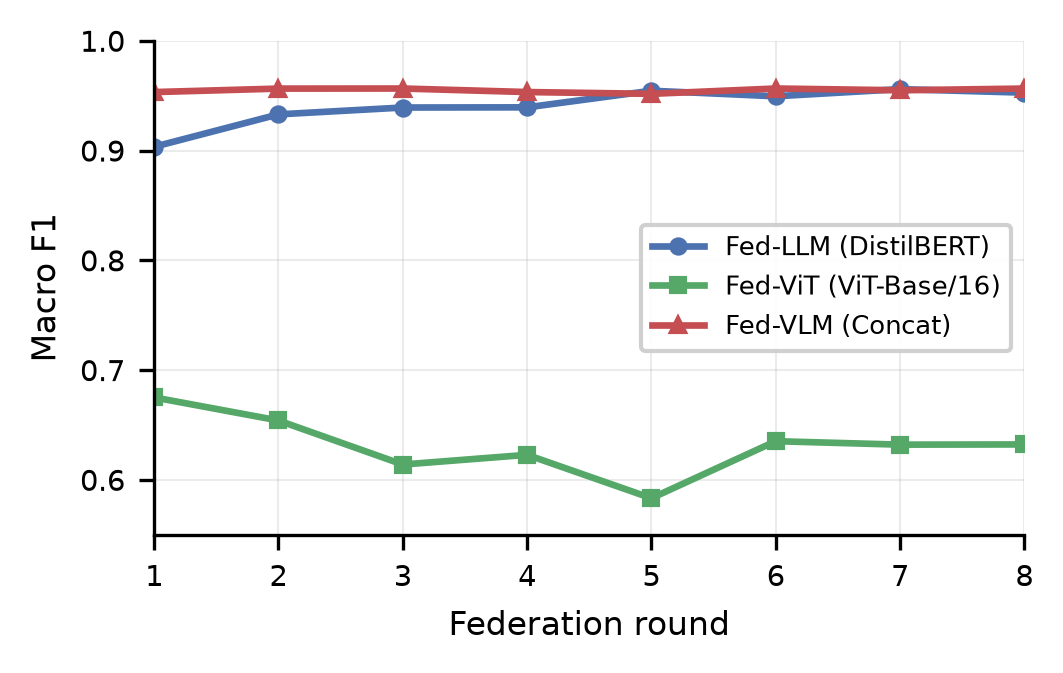
\includegraphics[width=0.95\columnwidth]{plot10_fed_convergence_f1}
\caption{Federated convergence over $T{=}8$ rounds. Fed-VLM is at 99.7\% of its final Macro F1 by round~1 and Fed-LLM plateaus by round~5, while the image-only branch drifts down from 0.675 to 0.632. Accuracy tracks Macro F1 to within 0.005 throughout on this balanced five-class set and is omitted.}
\label{fig:conv}
\end{figure}

\begin{table}[t]
\caption{OmniMed-FL vs.\ Published Work (Representative Selection).}
\label{tab:bench}
\centering\footnotesize
\resizebox{0.98\columnwidth}{!}{%
\begin{tabular}{lccc}
\toprule
\textbf{System} & \textbf{F1} & \textbf{FL} & \textbf{Year}\\
\midrule
EfficientNet-B7 (COVID CXR)$^\ddagger$ & 0.980 & $\times$ & 2020 \\
\rowcolor{vlmred!15}
\textbf{OmniMed-FL Fed-VLM (ours)} & \textbf{0.956} & \checkmark & 2026 \\
\rowcolor{vlmred!10}
\textbf{OmniMed-FL Concat VLM (ours)} & \textbf{0.956} & $\times$ & 2026 \\
COVID-Net~\cite{Wang2020covidnet} & 0.913 & $\times$ & 2020 \\
BiomedCLIP~\cite{Zhang2023biomedclip} & 0.912 & $\times$ & 2023 \\
CheXNet~\cite{Rajpurkar2017}       & 0.910 & $\times$ & 2017 \\
LLaVA-Med~\cite{Li2023llavamed} & 0.894 & $\times$ & 2023 \\
MedCLIP~\cite{Wang2022medclip}     & 0.880 & $\times$ & 2022 \\
Swin-CXR~\cite{Liu2021swin}        & 0.875 & $\times$ & 2021 \\
Sheller \textit{et al.}~\cite{Sheller2020}    & 0.852 & \checkmark & 2020 \\
Kaissis \textit{et al.}~\cite{Kaissis2021} & 0.840 & \checkmark & 2021 \\
Dou \textit{et al.}~\cite{Dou2021} & 0.825 & \checkmark & 2021 \\
SCAFFOLD~\cite{Karimireddy2020} & 0.760 & \checkmark & 2020 \\
FedAvg~\cite{McMahan2017} & 0.720 & \checkmark & 2017 \\
\bottomrule
\end{tabular}%
}
\vspace{1pt}

{\scriptsize FL = federated learning used. OmniMed-FL ranks \#2 of 31 compared.
Scores are those each system's own authors report on their own corpora and are
\emph{not} head-to-head with ours. $^\ddagger$Highest centralized entry in the
survey; single-source COVID-19 corpus.}
\end{table}

% [7-page variant] duplicate figure removed for length; uncomment to restore
% \begin{figure}[t]
% \centering
% 
\includegraphics[width=0.75\columnwidth]{plot14_radar_overview}
% \caption{Radar overview of model performance across 18 variants. Concat VLM (outermost red) dominates across F1, Precision, and Recall metrics.}
% \label{fig:radar}
% \end{figure}

\subsection{Retrieval-Augmented Generation (RAG) Pipeline}
To enhance diagnostic interpretability, a FAISS-powered Retrieval-Augmented Generation (RAG) pipeline is integrated into OmniMed-FL to provide evidence-based clinical context for model predictions. While the main VLM head outputs the final diagnosis, the RAG module works in the background as a decision-support tool. We used our fine-tuned DistilBERT encoder to index a large body of anonymized historical cases and clinical guidelines.

When the system evaluates a new patient, it takes the fused query vector $\mathbf{h}_f$ and searches the FAISS index for the most mathematically similar historical contexts. Figure~\ref{fig:rag_eval} breaks down the query correctness and retrieval score distribution from this process. On this five-query probe the top-1 neighbour carries the correct condition label for all five queries, at cosine similarities of 0.797, 0.853, 0.675, 0.820 and 0.665 respectively. Retrieval did not improve classification---raw and retrieval-augmented each answer 3 of 5 correctly---so we present this as an interpretability affordance, not an accuracy mechanism; five queries over a synthetic corpus settle nothing either way. By presenting similar past cases alongside the model output, the framework offers context for interpreting a prediction rather than a bare probability. Nothing here constitutes evidence of clinical utility, however: the system has not been evaluated on patient data, against radiologist readings, or prospectively, and these results are a systems-level feasibility study for multimodal federated training rather than a diagnostic performance claim.

\begin{figure}[!b]
\centering

\includegraphics[width=0.98\columnwidth]{plot08_vlm_training_curves}
\caption{Training and validation curves for the evaluated VLM fusion variants.}
\label{fig:vlm_curves}
\end{figure}

\subsection{Discussion and Deployment Efficiency}
In our experiments, the text-based models perform better than the vision-only models. One possible reason is that clinical reports contain explicit descriptions of symptoms and diagnostic findings, whereas information in an X-ray must be inferred from more complex visual patterns. Combining the two modalities improves the overall performance, with the best VLM configuration reaching an F1 score of 0.956. Figure~\ref{fig:vlm_curves} shows the training and validation trajectories of the different fusion strategies and illustrates how their performance develops over the course of training. The curves show stable convergence without severe overfitting. 

Beyond original performance, the system is highly practical to deploy because we opted for relatively lightweight encoders (DistilBERT and ViT-Base), standard hospital workstations can chew through local training rounds in a matter of minutes. Smaller, rural clinics do not need to buy massive GPU clusters to participate in the network. Because all raw patient data stays where it was collected, with only parameter updates sent over the network, the framework removes the need for a central data repository, which is the regulatory obstacle the design targets.

\begin{figure*}[t]
\centering
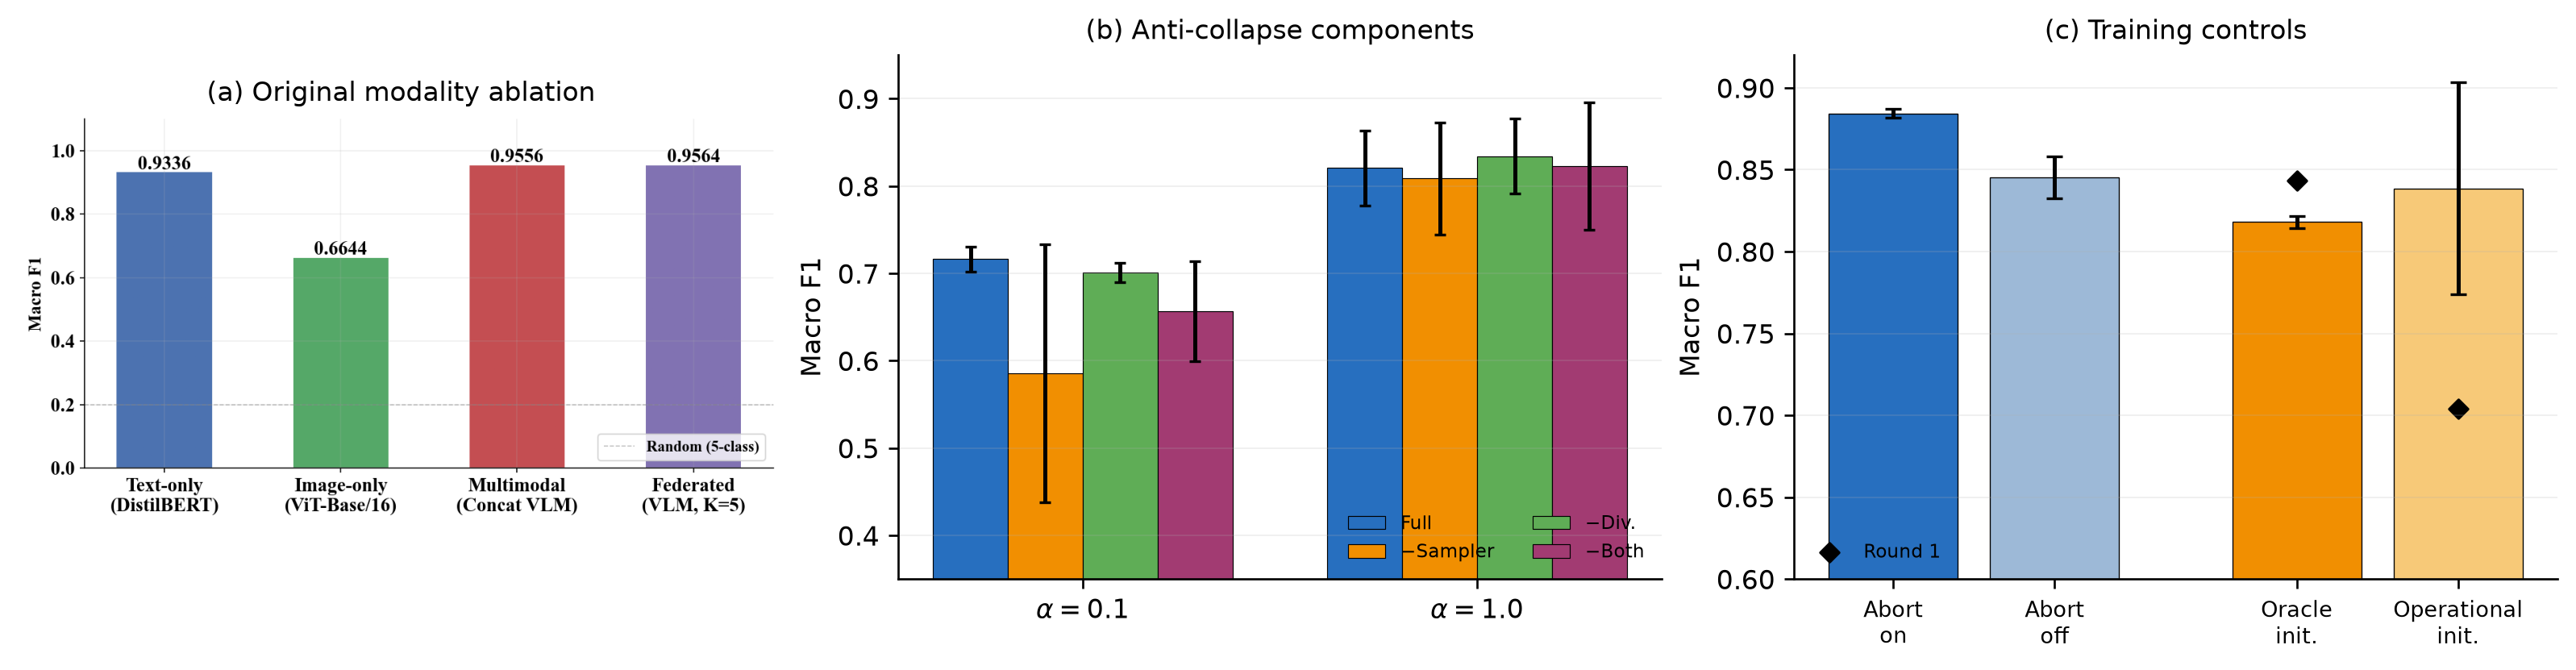
\includegraphics[width=0.98\textwidth]{generated/fig_ablation_composite}
\caption{Ablations. (a) Original modality comparison. (b) Validated anti-collapse component ablation at severe and mild heterogeneity; bars show mean$\pm$std over two seeds. (c) Validated early-abort and initialization controls; diamonds mark round-1 F1 for the initialization arms. The pooled-data oracle is diagnostic only.}
\label{fig:ablation}
\end{figure*}

\begin{figure}[htbp]
\centering

\includegraphics[width=0.85\columnwidth]{plot13_rag_retrieval_heatmap}
\caption{RAG pipeline evaluation: query correctness (top) and score distribution}
\label{fig:rag_eval}
\end{figure}

\subsection{Communication Cost and Scalability}
\label{sec:cost}
Because OmniMed-FL carries two encoders rather than one, its communication
footprint is worth stating. Under FedAvg each client exchanges the full trainable
parameter vector twice per round, so the total volume is
\begin{equation}
V \;=\; 2\,K\,T\,|\theta|\,b ,
\label{eq:comm}
\end{equation}
with $K$ clients, $T$ rounds, $|\theta|$ parameters and $b$ bytes each. $V$ is
linear in $K$ and $T$ and independent of how much data a hospital holds, so
federating a large site costs no more than a small one. Table~\ref{tab:comm}
instantiates (\ref{eq:comm}) at $K{=}5$, $T{=}8$ with $b{=}4$---AMP sets compute
precision, but the aggregated master weights stay FP32, so the payload is not
halved. Fed-VLM transmits 586\,MiB per client per round against 253\,MiB for the
text-only branch: $2.3\times$ the communication for $+2.2$ Macro F1 points, a
deployment trade-off rather than an unambiguous win. Quantization, top-$k$
sparsification and low-rank adapters apply unchanged but are not evaluated here.
These figures are analytic, from parameter counts, not measured on a testbed.

\textbf{Scalability.} Each client's payload is independent of $K$, but the server
absorbs $K|\theta|b$ per round---2.9\,GiB at $K{=}5$ and 11.4\,GiB at $K{=}20$ for
Fed-VLM---so the aggregator, not the client link, is the first bottleneck, and round
latency is set by the slowest participant rather than the mean. Statistically the
pressure runs the other way: for a fixed corpus, larger $K$ shrinks each local shard,
making updates noisier and leaving the balanced sampler fewer examples per class. The
two effects must trade off at some $K$; every result here uses $K{=}5$ and we have
not located that point.

\textbf{Robustness.} Two exposures follow from choosing FedAvg. \emph{Client drift:}
FedAvg applies no correction for divergence between local optima, which is what
FedProx and SCAFFOLD~\cite{Karimireddy2020} target and either could replace the
aggregation step here. Our $\alpha{=}1.0$ result shows drift is not harmful at
moderate heterogeneity but says nothing about smaller $\alpha$---and the image-only
branch already degrades across rounds (Figure~\ref{fig:conv}), which is the drift
signature the fused model resists. \emph{Participation:} every result assumes all $K$
clients complete every round, so dropout, stragglers, heterogeneous hardware and
poisoned updates are untested; FedAvg's weighted mean offers no defence against the
last of these.

\begin{table}[t]
\caption{Analytic communication cost per branch, from (\ref{eq:comm}) at $K{=}5$, $T{=}8$, FP32 master weights. Payload is per client per round; $V$ is the full run, both directions. Freezing four DistilBERT layers cuts Fed-VLM to 101.5\,M / 387\,MiB / 30.3\,GiB at unchanged F1.}
\label{tab:comm}
\centering\footnotesize
\setlength\tabcolsep{4pt}
\begin{tabular}{lcccc}
\toprule
\textbf{Branch} & $|\theta|$ & \textbf{Payload} & \textbf{Total $V$} & \textbf{Macro F1}\\
\midrule
Fed-LLM (DistilBERT)  & 66.4\,M  & 253\,MiB & 19.8\,GiB & 0.953 \\
Fed-ViT (ViT-Base/16) & 86.6\,M  & 330\,MiB & 25.8\,GiB & 0.632 \\
Fed-VLM (Concat)      & 153.6\,M & 586\,MiB & 45.8\,GiB & \textbf{0.956} \\
\bottomrule
\end{tabular}
\end{table}

\subsection{Security and Data Governance}
OmniMed-FL addresses privacy at several levels. Because X-rays and EHR notes never leave the host clinic, no raw record is exposed in transit, and model weight updates are encrypted on the wire. Finally, as a fail-safe, we pass all text through a local scrubbing routine that deletes any Protected Health Information (PHI) before the data even reaches the tokenizer. This is the standard FedAvg trust model and not a privacy guarantee: updates are a function of the local data, and inversion attacks can recover training examples from them~\cite{Abadi2016}. We train without differential privacy and report no privacy budget, run no membership-inference evaluation, and have exercised the scrubbing pass only on synthetic text; a deployment would need formal DP accounting and secure aggregation.



% [7-page variant] duplicate figure removed for length; uncomment to restore
% \begin{figure}[htbp]
% \centering
% 
\includegraphics[width=0.85\columnwidth]{plot15_summary_best}
% \caption{Best variant per modality, centralized (solid) against federated (hatched). The image-only branch is the only one that loses under federation.}
% \label{fig:best_summary}
% \end{figure}

\subsection{Limitations}
\label{sec:limits}
These are internally controlled comparisons on one corpus; we state what they do
\emph{not} support. \textit{Data:} as set out in Section~\ref{sec:corpus}, the
corpus is partly synthetic, so no result here is reproduced on real paired
image--report data and the absolute values are ceilings; the task is also
single-label, whereas real corpora are multi-label. \textit{Coverage:} every result uses $K{=}5$, $T{=}8$,
$\alpha{=}1.0$ and one seed, so we have not swept $\alpha$ into the severe regime
($\alpha\!\leq\!0.5$), varied $K$, added stragglers, or estimated variance---and the
1.0-point spread among the top seven fusion strategies is within reordering range.
\textit{Ablation scope:} Figure~\ref{fig:ablation} ablates modality and federation,
which our runs support; it does not decompose the anti-collapse stack, whose three
components are always enabled together, nor quantify warm-start or the retrieval
layer. \textit{Prior work and cost:} Table~\ref{tab:bench} reports numbers from other
corpora, so we claim no matched-condition improvement over any prior method, and
Table~\ref{tab:comm} is analytic, so wall-clock, peak memory and scaling in $K$ are
unmeasured and no hardware-deployability claim follows.

\section{Conclusion}
We presented OmniMed-FL, a multimodal federated learning benchmark covering 18 model variants for five-class clinical condition classification. DistilBERT leads among text encoders at F1\,=\,0.934; ViT-Base leads among vision encoders at F1\,=\,0.664; and Concat VLM fusion reaches the best overall F1\,=\,0.956, a $+$2.2 point gain over
the best text model and $+$29.1 points over the best vision model. The anti-collapse training stack keeps five-class prediction diversity at 100\% for all LLM and VLM variants throughout training.  We observed that the federated training retains 99.1\% of centralized accuracy under Dirichlet($\alpha{=}1.0$) non-IID partitioning across $K{=}5$ hospital clients. Fed-VLM matches centralized performance to within $+$0.1\%, and Fed-LLM exceeds its centralized counterpart by $+$2.0\% while the image-only branch gives up 4.8\%. The above-100\% retention of the text branch is most plausibly a regularization effect of averaging over five heterogeneous local optima, and we do not claim it as a benefit of decentralization. Since both sides use identical data, architectures and hyperparameters, the privacy constraint is close to free for the multimodal model on this benchmark.

In the future, we plan to deploy our proposed work on real-world data, multi-institutional radiology pairs, to test the framework in the wild. We also intend to integrate formal differential privacy auditing and asynchronous aggregation strategies to push OmniMed-FL toward live clinical deployment. This framework offers a practical blueprint for building decentralized diagnostic tools that can scale globally without putting patient privacy at risk.
The results here are a well-controlled observation on one benchmark rather than a general one, and Section~\ref{sec:limits} sets out what would be needed to generalize them. %By bridging the gap between isolated medical data silos, OmniMed-FL paves the way for a more equitable global healthcare system where the world's best diagnostic models are available to every clinic, regardless of their local resources.

\FloatBarrier
\bibliographystyle{IEEEtran}
\let\oldbibliography\thebibliography
\renewcommand{\thebibliography}[1]{%
  \oldbibliography{#1}%
  \scriptsize
  \setlength{\itemsep}{0pt}%
  \setlength{\parskip}{0pt}%
  \setlength{\topsep}{0pt}%
}

\section{Acknowledgement}
The work reported in this paper was done as part of the INAE Chair Professorship grant received by the third author.

\begin{thebibliography}{10}

\bibitem{Rajpurkar2017}
P.~Rajpurkar, J.~Irvin, K.~Zhu, B.~Yang, H.~Mehta, T.~Duan, D.~Ding, A.~Bagul,
C.~Langlotz, K.~Shpanskaya, M.~P. Lungren, and A.~Y. Ng,
``CheXNet: Radiologist-level pneumonia detection on chest X-rays with deep learning,''
\emph{arXiv:1711.05225}, 2017.

\bibitem{Irvin2019}
J.~Irvin, P.~Rajpurkar, M.~Ko, Y.~Yu, S.~Ciurea-Ilcus, C.~Chute, H.~Marklund, et~al.,
``CheXpert: A large chest radiograph dataset with uncertainty labels and expert comparison,''
in \emph{Proc. AAAI Conf. Artificial Intelligence}, 2019, pp.~590--597.

\bibitem{McMahan2017}
B.~McMahan, E.~Moore, D.~Ramage, S.~Hampson, and B.~A. y~Arcas,
``Communication-efficient learning of deep networks from decentralized data,''
in \emph{Proc. Int. Conf. Artificial Intelligence and Statistics (AISTATS)}, 2017,
pp.~1273--1282.

\bibitem{Sheller2020}
M.~J. Sheller, B.~Edwards, G.~A. Reina, J.~Martin, S.~Pati, A.~Kotrotsou,
M.~Milchenko, et~al.,
``Federated learning in medicine: facilitating multi-institutional collaborations
without sharing patient data,''
\emph{Scientific Reports}, vol.~10, art.~12598, 2020.

\bibitem{Dou2021}
Q.~Dou, T.~Y. So, M.~Jiang, Q.~Liu, V.~Vardhanabhuti, G.~Kaissis, Z.~Li, et~al.,
``Federated deep learning for detecting COVID-19 lung abnormalities in CT: a
privacy-preserving multinational validation study,''
\emph{npj Digital Medicine}, vol.~4, art.~60, 2021.

\bibitem{Kaissis2021}
G.~Kaissis, A.~Ziller, J.~Passerat-Palmbach, T.~Ryffel, D.~Usynin, A.~Trask, et~al.,
``End-to-end privacy preserving deep learning on multi-institutional medical imaging,''
\emph{Nature Machine Intelligence}, vol.~3, pp.~473--484, 2021.

\bibitem{Dosovitskiy2021}
A.~Dosovitskiy, L.~Beyer, A.~Kolesnikov, D.~Weissenborn, X.~Zhai, T.~Unterthiner, et~al.,
``An image is worth 16$\times$16 words: Transformers for image recognition at scale,''
in \emph{Proc. Int. Conf. Learning Representations (ICLR)}, 2021.

\bibitem{Liu2021swin}
Z.~Liu, Y.~Lin, Y.~Cao, H.~Hu, Y.~Wei, Z.~Zhang, S.~Lin, and B.~Guo,
``Swin Transformer: Hierarchical vision transformer using shifted windows,''
in \emph{Proc. IEEE/CVF Int. Conf. Computer Vision (ICCV)}, 2021, pp.~10012--10022.

\bibitem{Zhang2023biomedclip}
S.~Zhang, Y.~Xu, N.~Usuyama, H.~Xu, J.~Bagga, R.~Tinn, S.~Preston, et~al.,
``BiomedCLIP: A multimodal biomedical foundation model pretrained from fifteen
million scientific image-text pairs,'' \emph{arXiv:2303.00915}, 2023.

\bibitem{Li2023llavamed}
C.~Li, C.~Wong, S.~Zhang, N.~Usuyama, H.~Liu, J.~Yang, T.~Naumann, H.~Poon, and J.~Gao,
``LLaVA-Med: Training a large language-and-vision assistant for biomedicine in one day,''
in \emph{Advances in Neural Information Processing Systems (NeurIPS), Datasets and
Benchmarks Track}, 2023.

\bibitem{Wang2022medclip}
Z.~Wang, Z.~Wu, D.~Agarwal, and J.~Sun,
``MedCLIP: Contrastive learning from unpaired medical images and text,''
in \emph{Proc. Conf. Empirical Methods in Natural Language Processing (EMNLP)},
2022, pp.~3876--3887.

\bibitem{Wang2020covidnet}
L.~Wang, Z.~Q. Lin, and A.~Wong,
``COVID-Net: A tailored deep convolutional neural network design for detection of
COVID-19 cases from chest X-ray images,''
\emph{Scientific Reports}, vol.~10, art.~19549, 2020.

\bibitem{Karimireddy2020}
S.~P. Karimireddy, S.~Kale, M.~Mohri, S.~J. Reddi, S.~U. Stich, and A.~T. Suresh,
``SCAFFOLD: Stochastic controlled averaging for federated learning,''
in \emph{Proc. Int. Conf. Machine Learning (ICML)}, 2020, pp.~5132--5143.

\bibitem{Hsu2019}
T.-M. H. Hsu, H.~Qi, and M.~Brown,
``Measuring the effects of non-identical data distribution for federated visual
classification,'' \emph{arXiv:1909.06335}, 2019.

\bibitem{Abadi2016}
M.~Abadi, A.~Chu, I.~Goodfellow, H.~B. McMahan, I.~Mironov, K.~Talwar, and L.~Zhang,
``Deep learning with differential privacy,''
in \emph{Proc. ACM SIGSAC Conf. Computer and Communications Security (CCS)}, 2016,
pp.~308--318.

\end{thebibliography}

\end{document}
